\subsection*{Geo-Informations-Grundlagen}
Jeder Punkt auf der Erdkugel wird eindeutig durch die Kombination eines Breiten- und eines Längengrades definiert.
Breitengrade (Latitudes) liegen stets im Bereich von -90° (Süden) bis 90° (Norden). 0° beschreibt den Äquator.
Längengrade (Longitudes) werden von -180° (westlich) bis 180° (östlich) angegeben. Bei 0° befindet sich der Nullmeridian (Prime Meridian), welcher durch Greenwich (GB) verläuft.
Hierbei ergibt sich ein wesentliches mathematisches Problem.
Da -180° und +180° aufeinanderliegen, ist die rein mathematische Differenz zweier unmittelbar um diesen Meridian gelegenen Punkte größer als jede andere Differenz zweier Punkte.
Ein weiteres Problem ist die Uneinigkeit verschiedener Spezifikationen und Normen über die Reihenfolge der beiden Werte.
In diesem Projekt wird stets mit <longitude, latitude> gearbeitet.

\begin{center}
    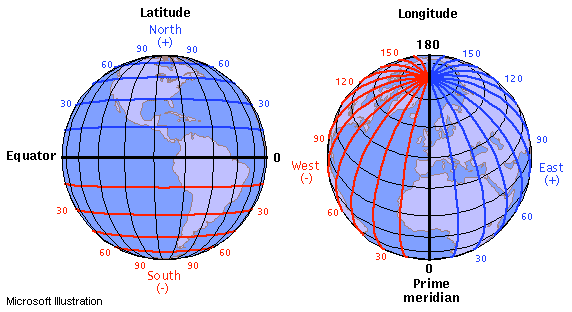
\includegraphics[width=\columnwidth]{images/lat-lon-world}
    \captionof{figure}{Visualisierung}
    \label{fig:REPLACE}
\end{center}

Für die Erfassung von Höhendaten gab es in der Vergangenheit verschiedene Projekte und Techniken.
Darunter fallen beispielsweise Lidar, Radar und Stereo-Photogrammetrie. Die so ermittelten Datensätze werden wiederum von verschiedenen Anbietern zur Verfügung gestellt.